\chapter{Výsledky}

\section{Ultratenké vrstvy La$_{2/3}$Sr$_{1/3}$MnO$_3$}
Spektra vzorků PLD můžeme srovnat s teoretickými hodnotami, které jsme vypočítali dle vztahu (\ref{teor kerr}). 
Výsledky jsou na obrázcích (\ref{sPLD189}) a (\ref{sPLD202}), na kterých je dobře vidět, že spektra získaná oběmy experimentálnímy 
metodami velmi dobře odpovídají teoretickému předpokladu. 

Na spektrech je také vidět, že modulační metoda 
dává pro energie nad 4.3 eV špatné výsledky. V této oblasti je vidět pokles obou ekeftů k nule, 
což je způsobeno postupnou ztrátou signálu na detektoru. Ta je způsobena 
snížením účinnosti fotonásobiče.

Dále je znatelný posun celého spekra. To je následek horšího spektrálního rozlišení monochromátoru. K tomu se ještě projevuje chybovost krokového motorku, který 
způsobuje další nepřesnost v určení vlnové délky světla.


\section{Kobaltové feritové tenké vrstvy}
Výsledky měření koblatových feritů jsou na obrázcích (\ref{sCoF-RT-A750}) a (\ref{sCoF-RT-A1100}). Z nich je dobře vidět, že vzorek je až do hodnoty 2.5 eV průhledný, protože na spektru vznikl interferenčí obrazec pro tenkou vrstvu. Výsledky metod se v této oblasti liší, protože úhel dopadu se u metod liší, což má za následek zdánlivý rozdíl 
v tloušťce vzorku. 

Nad 2.5 eV je spektrum už typické pro ferity. Konkrétně má velmi podobné spektrum má i lithný a mědnatý ferit. \cite{ferity} 

Dále je vidět vliv depoziční teploty na spektrum vzorku. Při vysokých teplotách totiž zřejmě dochází k materiálovým změnám, které mají za následek zeslabení magnetických efektů.

\section{Heuslerovy slitiny}
Spektra vzorků Heuslerových slitin jsou na obrázcích (\ref{sCoFeSi1}) a (\ref{sCoFeSi2}). Rozdílná velikost amplitud efektů je daná použitím různých magnetů. 
Magnet první z metod totiž nevytváří dostatečně velké pole pro nasycení vzorku. Porovnáním tvarů spekter však vidíme, že si výsledky obou metod odpovídají.

Ze spekter je také dobře vidět, že vetší přítomnost železa proti kobaltu ve vzorku má za následek větší efekt.



\begin{figure}
% GNUPLOT: LaTeX picture with Postscript
\begingroup
  \makeatletter
  \providecommand\color[2][]{%
    \GenericError{(gnuplot) \space\space\space\@spaces}{%
      Package color not loaded in conjunction with
      terminal option `colourtext'%
    }{See the gnuplot documentation for explanation.%
    }{Either use 'blacktext' in gnuplot or load the package
      color.sty in LaTeX.}%
    \renewcommand\color[2][]{}%
  }%
  \providecommand\includegraphics[2][]{%
    \GenericError{(gnuplot) \space\space\space\@spaces}{%
      Package graphicx or graphics not loaded%
    }{See the gnuplot documentation for explanation.%
    }{The gnuplot epslatex terminal needs graphicx.sty or graphics.sty.}%
    \renewcommand\includegraphics[2][]{}%
  }%
  \providecommand\rotatebox[2]{#2}%
  \@ifundefined{ifGPcolor}{%
    \newif\ifGPcolor
    \GPcolorfalse
  }{}%
  \@ifundefined{ifGPblacktext}{%
    \newif\ifGPblacktext
    \GPblacktexttrue
  }{}%
  % define a \g@addto@macro without @ in the name:
  \let\gplgaddtomacro\g@addto@macro
  % define empty templates for all commands taking text:
  \gdef\gplbacktext{}%
  \gdef\gplfronttext{}%
  \makeatother
  \ifGPblacktext
    % no textcolor at all
    \def\colorrgb#1{}%
    \def\colorgray#1{}%
  \else
    % gray or color?
    \ifGPcolor
      \def\colorrgb#1{\color[rgb]{#1}}%
      \def\colorgray#1{\color[gray]{#1}}%
      \expandafter\def\csname LTw\endcsname{\color{white}}%
      \expandafter\def\csname LTb\endcsname{\color{black}}%
      \expandafter\def\csname LTa\endcsname{\color{black}}%
      \expandafter\def\csname LT0\endcsname{\color[rgb]{1,0,0}}%
      \expandafter\def\csname LT1\endcsname{\color[rgb]{0,1,0}}%
      \expandafter\def\csname LT2\endcsname{\color[rgb]{0,0,1}}%
      \expandafter\def\csname LT3\endcsname{\color[rgb]{1,0,1}}%
      \expandafter\def\csname LT4\endcsname{\color[rgb]{0,1,1}}%
      \expandafter\def\csname LT5\endcsname{\color[rgb]{1,1,0}}%
      \expandafter\def\csname LT6\endcsname{\color[rgb]{0,0,0}}%
      \expandafter\def\csname LT7\endcsname{\color[rgb]{1,0.3,0}}%
      \expandafter\def\csname LT8\endcsname{\color[rgb]{0.5,0.5,0.5}}%
    \else
      % gray
      \def\colorrgb#1{\color{black}}%
      \def\colorgray#1{\color[gray]{#1}}%
      \expandafter\def\csname LTw\endcsname{\color{white}}%
      \expandafter\def\csname LTb\endcsname{\color{black}}%
      \expandafter\def\csname LTa\endcsname{\color{black}}%
      \expandafter\def\csname LT0\endcsname{\color{black}}%
      \expandafter\def\csname LT1\endcsname{\color{black}}%
      \expandafter\def\csname LT2\endcsname{\color{black}}%
      \expandafter\def\csname LT3\endcsname{\color{black}}%
      \expandafter\def\csname LT4\endcsname{\color{black}}%
      \expandafter\def\csname LT5\endcsname{\color{black}}%
      \expandafter\def\csname LT6\endcsname{\color{black}}%
      \expandafter\def\csname LT7\endcsname{\color{black}}%
      \expandafter\def\csname LT8\endcsname{\color{black}}%
    \fi
  \fi
  \setlength{\unitlength}{0.0500bp}%
  \begin{picture}(7200.00,5040.00)%
    \gplgaddtomacro\gplbacktext{%
      \csname LTb\endcsname%
      \put(1210,704){\makebox(0,0)[r]{\strut{}-0.2}}%
      \put(1210,1213){\makebox(0,0)[r]{\strut{}-0.15}}%
      \put(1210,1722){\makebox(0,0)[r]{\strut{}-0.1}}%
      \put(1210,2231){\makebox(0,0)[r]{\strut{}-0.05}}%
      \put(1210,2739){\makebox(0,0)[r]{\strut{} 0}}%
      \put(1210,3248){\makebox(0,0)[r]{\strut{} 0.05}}%
      \put(1210,3757){\makebox(0,0)[r]{\strut{} 0.1}}%
      \put(1210,4266){\makebox(0,0)[r]{\strut{} 0.15}}%
      \put(1210,4775){\makebox(0,0)[r]{\strut{} 0.2}}%
      \put(1496,484){\makebox(0,0){\strut{} 1.5}}%
      \put(2263,484){\makebox(0,0){\strut{} 2}}%
      \put(3031,484){\makebox(0,0){\strut{} 2.5}}%
      \put(3798,484){\makebox(0,0){\strut{} 3}}%
      \put(4566,484){\makebox(0,0){\strut{} 3.5}}%
      \put(5334,484){\makebox(0,0){\strut{} 4}}%
      \put(6101,484){\makebox(0,0){\strut{} 4.5}}%
      \put(6869,484){\makebox(0,0){\strut{} 5}}%
      \put(308,2739){\rotatebox{-270}{\makebox(0,0){\strut{}Polární Kerrův jev [deg.]}}}%
      \put(4105,154){\makebox(0,0){\strut{}$E$/eV}}%
    }%
    \gplgaddtomacro\gplfronttext{%
      \csname LTb\endcsname%
      \put(5882,4602){\makebox(0,0)[r]{\strut{}$\theta^1_K$}}%
      \csname LTb\endcsname%
      \put(5882,4382){\makebox(0,0)[r]{\strut{}$\epsilon^1_K$}}%
      \csname LTb\endcsname%
      \put(5882,4162){\makebox(0,0)[r]{\strut{}$\theta^2_K$}}%
      \csname LTb\endcsname%
      \put(5882,3942){\makebox(0,0)[r]{\strut{}$\epsilon^2_K$}}%
    }%
    \gplbacktext
    \put(0,0){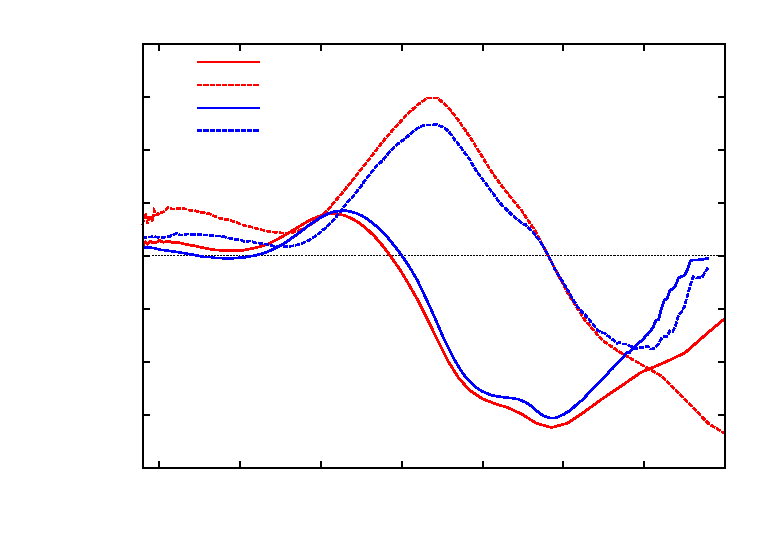
\includegraphics{grafy/PLD186}}%
    \gplfronttext
  \end{picture}%
\endgroup

\caption{Spektrum vzorku PLD186}
\label{sPLD189}
\end{figure}

\begin{figure}
% GNUPLOT: LaTeX picture with Postscript
\begingroup
  \makeatletter
  \providecommand\color[2][]{%
    \GenericError{(gnuplot) \space\space\space\@spaces}{%
      Package color not loaded in conjunction with
      terminal option `colourtext'%
    }{See the gnuplot documentation for explanation.%
    }{Either use 'blacktext' in gnuplot or load the package
      color.sty in LaTeX.}%
    \renewcommand\color[2][]{}%
  }%
  \providecommand\includegraphics[2][]{%
    \GenericError{(gnuplot) \space\space\space\@spaces}{%
      Package graphicx or graphics not loaded%
    }{See the gnuplot documentation for explanation.%
    }{The gnuplot epslatex terminal needs graphicx.sty or graphics.sty.}%
    \renewcommand\includegraphics[2][]{}%
  }%
  \providecommand\rotatebox[2]{#2}%
  \@ifundefined{ifGPcolor}{%
    \newif\ifGPcolor
    \GPcolorfalse
  }{}%
  \@ifundefined{ifGPblacktext}{%
    \newif\ifGPblacktext
    \GPblacktexttrue
  }{}%
  % define a \g@addto@macro without @ in the name:
  \let\gplgaddtomacro\g@addto@macro
  % define empty templates for all commands taking text:
  \gdef\gplbacktext{}%
  \gdef\gplfronttext{}%
  \makeatother
  \ifGPblacktext
    % no textcolor at all
    \def\colorrgb#1{}%
    \def\colorgray#1{}%
  \else
    % gray or color?
    \ifGPcolor
      \def\colorrgb#1{\color[rgb]{#1}}%
      \def\colorgray#1{\color[gray]{#1}}%
      \expandafter\def\csname LTw\endcsname{\color{white}}%
      \expandafter\def\csname LTb\endcsname{\color{black}}%
      \expandafter\def\csname LTa\endcsname{\color{black}}%
      \expandafter\def\csname LT0\endcsname{\color[rgb]{1,0,0}}%
      \expandafter\def\csname LT1\endcsname{\color[rgb]{0,1,0}}%
      \expandafter\def\csname LT2\endcsname{\color[rgb]{0,0,1}}%
      \expandafter\def\csname LT3\endcsname{\color[rgb]{1,0,1}}%
      \expandafter\def\csname LT4\endcsname{\color[rgb]{0,1,1}}%
      \expandafter\def\csname LT5\endcsname{\color[rgb]{1,1,0}}%
      \expandafter\def\csname LT6\endcsname{\color[rgb]{0,0,0}}%
      \expandafter\def\csname LT7\endcsname{\color[rgb]{1,0.3,0}}%
      \expandafter\def\csname LT8\endcsname{\color[rgb]{0.5,0.5,0.5}}%
    \else
      % gray
      \def\colorrgb#1{\color{black}}%
      \def\colorgray#1{\color[gray]{#1}}%
      \expandafter\def\csname LTw\endcsname{\color{white}}%
      \expandafter\def\csname LTb\endcsname{\color{black}}%
      \expandafter\def\csname LTa\endcsname{\color{black}}%
      \expandafter\def\csname LT0\endcsname{\color{black}}%
      \expandafter\def\csname LT1\endcsname{\color{black}}%
      \expandafter\def\csname LT2\endcsname{\color{black}}%
      \expandafter\def\csname LT3\endcsname{\color{black}}%
      \expandafter\def\csname LT4\endcsname{\color{black}}%
      \expandafter\def\csname LT5\endcsname{\color{black}}%
      \expandafter\def\csname LT6\endcsname{\color{black}}%
      \expandafter\def\csname LT7\endcsname{\color{black}}%
      \expandafter\def\csname LT8\endcsname{\color{black}}%
    \fi
  \fi
  \setlength{\unitlength}{0.0500bp}%
  \begin{picture}(7200.00,5040.00)%
    \gplgaddtomacro\gplbacktext{%
      \csname LTb\endcsname%
      \put(990,704){\makebox(0,0)[r]{\strut{}-0.2}}%
      \put(990,1213){\makebox(0,0)[r]{\strut{}-0.15}}%
      \put(990,1722){\makebox(0,0)[r]{\strut{}-0.1}}%
      \put(990,2231){\makebox(0,0)[r]{\strut{}-0.05}}%
      \put(990,2739){\makebox(0,0)[r]{\strut{} 0}}%
      \put(990,3248){\makebox(0,0)[r]{\strut{} 0.05}}%
      \put(990,3757){\makebox(0,0)[r]{\strut{} 0.1}}%
      \put(990,4266){\makebox(0,0)[r]{\strut{} 0.15}}%
      \put(990,4775){\makebox(0,0)[r]{\strut{} 0.2}}%
      \put(1282,484){\makebox(0,0){\strut{} 1.5}}%
      \put(2080,484){\makebox(0,0){\strut{} 2}}%
      \put(2878,484){\makebox(0,0){\strut{} 2.5}}%
      \put(3676,484){\makebox(0,0){\strut{} 3}}%
      \put(4474,484){\makebox(0,0){\strut{} 3.5}}%
      \put(5273,484){\makebox(0,0){\strut{} 4}}%
      \put(6071,484){\makebox(0,0){\strut{} 4.5}}%
      \put(6869,484){\makebox(0,0){\strut{} 5}}%
      \put(308,2739){\rotatebox{-270}{\makebox(0,0){\strut{}}}}%
      \put(3995,154){\makebox(0,0){\strut{}$E$/eV}}%
    }%
    \gplgaddtomacro\gplfronttext{%
      \csname LTb\endcsname%
      \put(3102,4602){\makebox(0,0)[r]{\strut{}$\theta^1_K$}}%
      \csname LTb\endcsname%
      \put(3102,4382){\makebox(0,0)[r]{\strut{}$\epsilon^1_K$}}%
    }%
    \gplbacktext
    \put(0,0){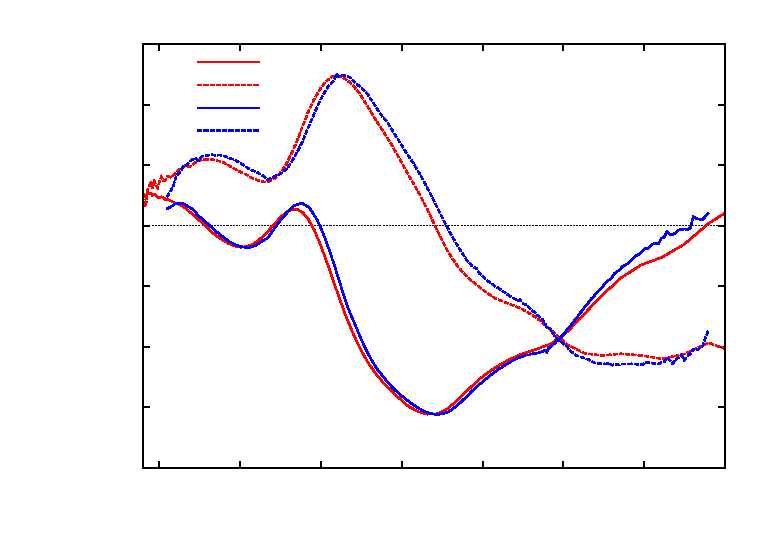
\includegraphics{PLD202}}%
    \gplfronttext
  \end{picture}%
\endgroup

\caption{Spektrum vzorku PLD202}
\label{sPLD202}
\end{figure}

\begin{figure}
% GNUPLOT: LaTeX picture with Postscript
\begingroup
  \makeatletter
  \providecommand\color[2][]{%
    \GenericError{(gnuplot) \space\space\space\@spaces}{%
      Package color not loaded in conjunction with
      terminal option `colourtext'%
    }{See the gnuplot documentation for explanation.%
    }{Either use 'blacktext' in gnuplot or load the package
      color.sty in LaTeX.}%
    \renewcommand\color[2][]{}%
  }%
  \providecommand\includegraphics[2][]{%
    \GenericError{(gnuplot) \space\space\space\@spaces}{%
      Package graphicx or graphics not loaded%
    }{See the gnuplot documentation for explanation.%
    }{The gnuplot epslatex terminal needs graphicx.sty or graphics.sty.}%
    \renewcommand\includegraphics[2][]{}%
  }%
  \providecommand\rotatebox[2]{#2}%
  \@ifundefined{ifGPcolor}{%
    \newif\ifGPcolor
    \GPcolortrue
  }{}%
  \@ifundefined{ifGPblacktext}{%
    \newif\ifGPblacktext
    \GPblacktexttrue
  }{}%
  % define a \g@addto@macro without @ in the name:
  \let\gplgaddtomacro\g@addto@macro
  % define empty templates for all commands taking text:
  \gdef\gplbacktext{}%
  \gdef\gplfronttext{}%
  \makeatother
  \ifGPblacktext
    % no textcolor at all
    \def\colorrgb#1{}%
    \def\colorgray#1{}%
  \else
    % gray or color?
    \ifGPcolor
      \def\colorrgb#1{\color[rgb]{#1}}%
      \def\colorgray#1{\color[gray]{#1}}%
      \expandafter\def\csname LTw\endcsname{\color{white}}%
      \expandafter\def\csname LTb\endcsname{\color{black}}%
      \expandafter\def\csname LTa\endcsname{\color{black}}%
      \expandafter\def\csname LT0\endcsname{\color[rgb]{1,0,0}}%
      \expandafter\def\csname LT1\endcsname{\color[rgb]{0,1,0}}%
      \expandafter\def\csname LT2\endcsname{\color[rgb]{0,0,1}}%
      \expandafter\def\csname LT3\endcsname{\color[rgb]{1,0,1}}%
      \expandafter\def\csname LT4\endcsname{\color[rgb]{0,1,1}}%
      \expandafter\def\csname LT5\endcsname{\color[rgb]{1,1,0}}%
      \expandafter\def\csname LT6\endcsname{\color[rgb]{0,0,0}}%
      \expandafter\def\csname LT7\endcsname{\color[rgb]{1,0.3,0}}%
      \expandafter\def\csname LT8\endcsname{\color[rgb]{0.5,0.5,0.5}}%
    \else
      % gray
      \def\colorrgb#1{\color{black}}%
      \def\colorgray#1{\color[gray]{#1}}%
      \expandafter\def\csname LTw\endcsname{\color{white}}%
      \expandafter\def\csname LTb\endcsname{\color{black}}%
      \expandafter\def\csname LTa\endcsname{\color{black}}%
      \expandafter\def\csname LT0\endcsname{\color{black}}%
      \expandafter\def\csname LT1\endcsname{\color{black}}%
      \expandafter\def\csname LT2\endcsname{\color{black}}%
      \expandafter\def\csname LT3\endcsname{\color{black}}%
      \expandafter\def\csname LT4\endcsname{\color{black}}%
      \expandafter\def\csname LT5\endcsname{\color{black}}%
      \expandafter\def\csname LT6\endcsname{\color{black}}%
      \expandafter\def\csname LT7\endcsname{\color{black}}%
      \expandafter\def\csname LT8\endcsname{\color{black}}%
    \fi
  \fi
  \setlength{\unitlength}{0.0500bp}%
  \begin{picture}(7200.00,5040.00)%
    \gplgaddtomacro\gplbacktext{%
      \csname LTb\endcsname%
      \put(946,704){\makebox(0,0)[r]{\strut{}-0.6}}%
      \put(946,1383){\makebox(0,0)[r]{\strut{}-0.4}}%
      \put(946,2061){\makebox(0,0)[r]{\strut{}-0.2}}%
      \put(946,2740){\makebox(0,0)[r]{\strut{} 0}}%
      \put(946,3418){\makebox(0,0)[r]{\strut{} 0.2}}%
      \put(946,4097){\makebox(0,0)[r]{\strut{} 0.4}}%
      \put(946,4775){\makebox(0,0)[r]{\strut{} 0.6}}%
      \put(1257,484){\makebox(0,0){\strut{} 1.5}}%
      \put(2151,484){\makebox(0,0){\strut{} 2}}%
      \put(3046,484){\makebox(0,0){\strut{} 2.5}}%
      \put(3941,484){\makebox(0,0){\strut{} 3}}%
      \put(4835,484){\makebox(0,0){\strut{} 3.5}}%
      \put(5730,484){\makebox(0,0){\strut{} 4}}%
      \put(6624,484){\makebox(0,0){\strut{} 4.5}}%
      \csname LTb\endcsname%
      \put(176,2739){\rotatebox{-270}{\makebox(0,0){\strut{}Polární Kerrův jev [deg.]}}}%
      \put(3940,154){\makebox(0,0){\strut{}$E$ [eV]}}%
    }%
    \gplgaddtomacro\gplfronttext{%
      \csname LTb\endcsname%
      \put(5816,4602){\makebox(0,0)[r]{\strut{}$\theta_K$}}%
      \csname LTb\endcsname%
      \put(5816,4382){\makebox(0,0)[r]{\strut{}$\epsilon_K$}}%
      \csname LTb\endcsname%
      \put(5816,4162){\makebox(0,0)[r]{\strut{}$\theta_K$}}%
      \csname LTb\endcsname%
      \put(5816,3942){\makebox(0,0)[r]{\strut{}$\epsilon_K$}}%
    }%
    \gplbacktext
    \put(0,0){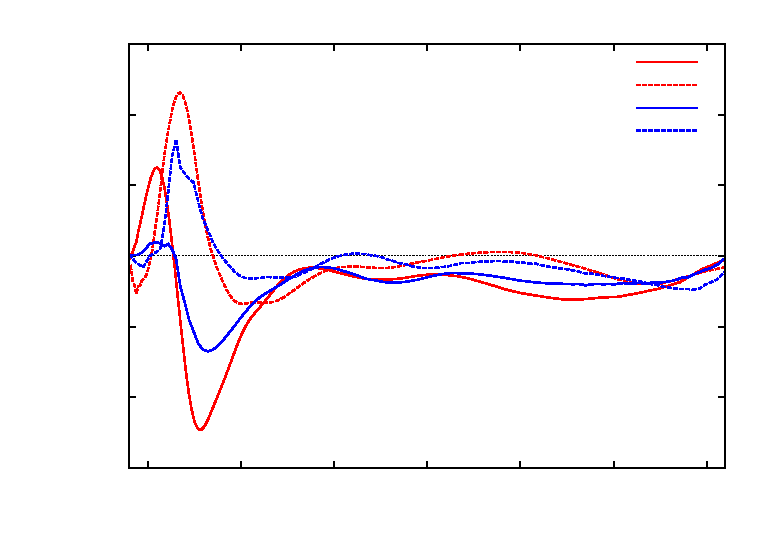
\includegraphics{CoF-RT-A750}}%
    \gplfronttext
  \end{picture}%
\endgroup

\caption{Spektrum vzorku CoF-RT-A750}
\label{sCoF-RT-A750}
\end{figure}

\begin{figure}
% GNUPLOT: LaTeX picture with Postscript
\begingroup
  \makeatletter
  \providecommand\color[2][]{%
    \GenericError{(gnuplot) \space\space\space\@spaces}{%
      Package color not loaded in conjunction with
      terminal option `colourtext'%
    }{See the gnuplot documentation for explanation.%
    }{Either use 'blacktext' in gnuplot or load the package
      color.sty in LaTeX.}%
    \renewcommand\color[2][]{}%
  }%
  \providecommand\includegraphics[2][]{%
    \GenericError{(gnuplot) \space\space\space\@spaces}{%
      Package graphicx or graphics not loaded%
    }{See the gnuplot documentation for explanation.%
    }{The gnuplot epslatex terminal needs graphicx.sty or graphics.sty.}%
    \renewcommand\includegraphics[2][]{}%
  }%
  \providecommand\rotatebox[2]{#2}%
  \@ifundefined{ifGPcolor}{%
    \newif\ifGPcolor
    \GPcolorfalse
  }{}%
  \@ifundefined{ifGPblacktext}{%
    \newif\ifGPblacktext
    \GPblacktexttrue
  }{}%
  % define a \g@addto@macro without @ in the name:
  \let\gplgaddtomacro\g@addto@macro
  % define empty templates for all commands taking text:
  \gdef\gplbacktext{}%
  \gdef\gplfronttext{}%
  \makeatother
  \ifGPblacktext
    % no textcolor at all
    \def\colorrgb#1{}%
    \def\colorgray#1{}%
  \else
    % gray or color?
    \ifGPcolor
      \def\colorrgb#1{\color[rgb]{#1}}%
      \def\colorgray#1{\color[gray]{#1}}%
      \expandafter\def\csname LTw\endcsname{\color{white}}%
      \expandafter\def\csname LTb\endcsname{\color{black}}%
      \expandafter\def\csname LTa\endcsname{\color{black}}%
      \expandafter\def\csname LT0\endcsname{\color[rgb]{1,0,0}}%
      \expandafter\def\csname LT1\endcsname{\color[rgb]{0,1,0}}%
      \expandafter\def\csname LT2\endcsname{\color[rgb]{0,0,1}}%
      \expandafter\def\csname LT3\endcsname{\color[rgb]{1,0,1}}%
      \expandafter\def\csname LT4\endcsname{\color[rgb]{0,1,1}}%
      \expandafter\def\csname LT5\endcsname{\color[rgb]{1,1,0}}%
      \expandafter\def\csname LT6\endcsname{\color[rgb]{0,0,0}}%
      \expandafter\def\csname LT7\endcsname{\color[rgb]{1,0.3,0}}%
      \expandafter\def\csname LT8\endcsname{\color[rgb]{0.5,0.5,0.5}}%
    \else
      % gray
      \def\colorrgb#1{\color{black}}%
      \def\colorgray#1{\color[gray]{#1}}%
      \expandafter\def\csname LTw\endcsname{\color{white}}%
      \expandafter\def\csname LTb\endcsname{\color{black}}%
      \expandafter\def\csname LTa\endcsname{\color{black}}%
      \expandafter\def\csname LT0\endcsname{\color{black}}%
      \expandafter\def\csname LT1\endcsname{\color{black}}%
      \expandafter\def\csname LT2\endcsname{\color{black}}%
      \expandafter\def\csname LT3\endcsname{\color{black}}%
      \expandafter\def\csname LT4\endcsname{\color{black}}%
      \expandafter\def\csname LT5\endcsname{\color{black}}%
      \expandafter\def\csname LT6\endcsname{\color{black}}%
      \expandafter\def\csname LT7\endcsname{\color{black}}%
      \expandafter\def\csname LT8\endcsname{\color{black}}%
    \fi
  \fi
  \setlength{\unitlength}{0.0500bp}%
  \begin{picture}(7200.00,5040.00)%
    \gplgaddtomacro\gplbacktext{%
      \csname LTb\endcsname%
      \put(1078,704){\makebox(0,0)[r]{\strut{}-0.4}}%
      \put(1078,1213){\makebox(0,0)[r]{\strut{}-0.3}}%
      \put(1078,1722){\makebox(0,0)[r]{\strut{}-0.2}}%
      \put(1078,2231){\makebox(0,0)[r]{\strut{}-0.1}}%
      \put(1078,2739){\makebox(0,0)[r]{\strut{} 0}}%
      \put(1078,3248){\makebox(0,0)[r]{\strut{} 0.1}}%
      \put(1078,3757){\makebox(0,0)[r]{\strut{} 0.2}}%
      \put(1078,4266){\makebox(0,0)[r]{\strut{} 0.3}}%
      \put(1078,4775){\makebox(0,0)[r]{\strut{} 0.4}}%
      \put(1367,484){\makebox(0,0){\strut{} 1.5}}%
      \put(2153,484){\makebox(0,0){\strut{} 2}}%
      \put(2939,484){\makebox(0,0){\strut{} 2.5}}%
      \put(3725,484){\makebox(0,0){\strut{} 3}}%
      \put(4511,484){\makebox(0,0){\strut{} 3.5}}%
      \put(5297,484){\makebox(0,0){\strut{} 4}}%
      \put(6083,484){\makebox(0,0){\strut{} 4.5}}%
      \put(6869,484){\makebox(0,0){\strut{} 5}}%
      \put(308,2739){\rotatebox{-270}{\makebox(0,0){\strut{}Polární Kerrův jev [deg.]}}}%
      \put(4039,154){\makebox(0,0){\strut{}$E$/eV}}%
    }%
    \gplgaddtomacro\gplfronttext{%
      \csname LTb\endcsname%
      \put(5882,4602){\makebox(0,0)[r]{\strut{}$\theta^1_K$}}%
      \csname LTb\endcsname%
      \put(5882,4382){\makebox(0,0)[r]{\strut{}$\epsilon^1_K$}}%
      \csname LTb\endcsname%
      \put(5882,4162){\makebox(0,0)[r]{\strut{}$\theta^2_K$}}%
      \csname LTb\endcsname%
      \put(5882,3942){\makebox(0,0)[r]{\strut{}$\epsilon^2_K$}}%
    }%
    \gplbacktext
    \put(0,0){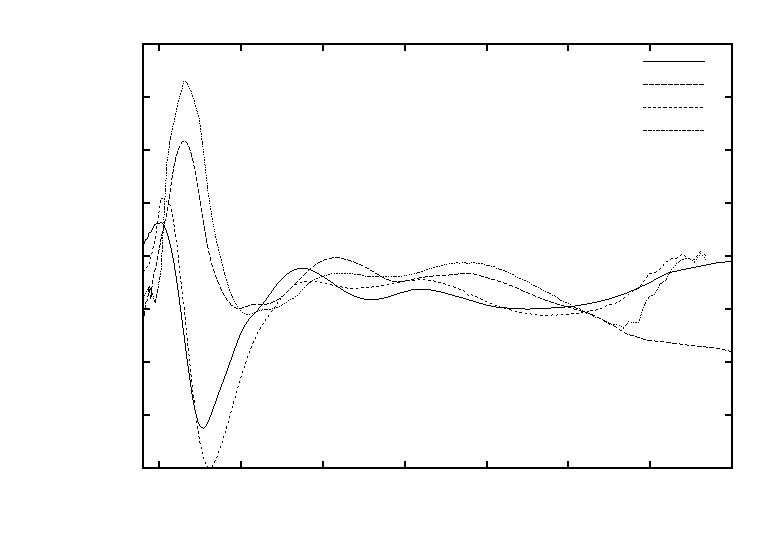
\includegraphics{grafy/CoF-RT-A1100}}%
    \gplfronttext
  \end{picture}%
\endgroup

\caption{Spektrum vzorku CoF-RT-A1100}
\label{sCoF-RT-A1100}
\end{figure}

\begin{figure}
% GNUPLOT: LaTeX picture with Postscript
\begingroup
  \makeatletter
  \providecommand\color[2][]{%
    \GenericError{(gnuplot) \space\space\space\@spaces}{%
      Package color not loaded in conjunction with
      terminal option `colourtext'%
    }{See the gnuplot documentation for explanation.%
    }{Either use 'blacktext' in gnuplot or load the package
      color.sty in LaTeX.}%
    \renewcommand\color[2][]{}%
  }%
  \providecommand\includegraphics[2][]{%
    \GenericError{(gnuplot) \space\space\space\@spaces}{%
      Package graphicx or graphics not loaded%
    }{See the gnuplot documentation for explanation.%
    }{The gnuplot epslatex terminal needs graphicx.sty or graphics.sty.}%
    \renewcommand\includegraphics[2][]{}%
  }%
  \providecommand\rotatebox[2]{#2}%
  \@ifundefined{ifGPcolor}{%
    \newif\ifGPcolor
    \GPcolorfalse
  }{}%
  \@ifundefined{ifGPblacktext}{%
    \newif\ifGPblacktext
    \GPblacktexttrue
  }{}%
  % define a \g@addto@macro without @ in the name:
  \let\gplgaddtomacro\g@addto@macro
  % define empty templates for all commands taking text:
  \gdef\gplbacktext{}%
  \gdef\gplfronttext{}%
  \makeatother
  \ifGPblacktext
    % no textcolor at all
    \def\colorrgb#1{}%
    \def\colorgray#1{}%
  \else
    % gray or color?
    \ifGPcolor
      \def\colorrgb#1{\color[rgb]{#1}}%
      \def\colorgray#1{\color[gray]{#1}}%
      \expandafter\def\csname LTw\endcsname{\color{white}}%
      \expandafter\def\csname LTb\endcsname{\color{black}}%
      \expandafter\def\csname LTa\endcsname{\color{black}}%
      \expandafter\def\csname LT0\endcsname{\color[rgb]{1,0,0}}%
      \expandafter\def\csname LT1\endcsname{\color[rgb]{0,1,0}}%
      \expandafter\def\csname LT2\endcsname{\color[rgb]{0,0,1}}%
      \expandafter\def\csname LT3\endcsname{\color[rgb]{1,0,1}}%
      \expandafter\def\csname LT4\endcsname{\color[rgb]{0,1,1}}%
      \expandafter\def\csname LT5\endcsname{\color[rgb]{1,1,0}}%
      \expandafter\def\csname LT6\endcsname{\color[rgb]{0,0,0}}%
      \expandafter\def\csname LT7\endcsname{\color[rgb]{1,0.3,0}}%
      \expandafter\def\csname LT8\endcsname{\color[rgb]{0.5,0.5,0.5}}%
    \else
      % gray
      \def\colorrgb#1{\color{black}}%
      \def\colorgray#1{\color[gray]{#1}}%
      \expandafter\def\csname LTw\endcsname{\color{white}}%
      \expandafter\def\csname LTb\endcsname{\color{black}}%
      \expandafter\def\csname LTa\endcsname{\color{black}}%
      \expandafter\def\csname LT0\endcsname{\color{black}}%
      \expandafter\def\csname LT1\endcsname{\color{black}}%
      \expandafter\def\csname LT2\endcsname{\color{black}}%
      \expandafter\def\csname LT3\endcsname{\color{black}}%
      \expandafter\def\csname LT4\endcsname{\color{black}}%
      \expandafter\def\csname LT5\endcsname{\color{black}}%
      \expandafter\def\csname LT6\endcsname{\color{black}}%
      \expandafter\def\csname LT7\endcsname{\color{black}}%
      \expandafter\def\csname LT8\endcsname{\color{black}}%
    \fi
  \fi
  \setlength{\unitlength}{0.0500bp}%
  \begin{picture}(7200.00,5040.00)%
    \gplgaddtomacro\gplbacktext{%
      \csname LTb\endcsname%
      \put(1122,704){\makebox(0,0)[r]{\strut{}-0.008}}%
      \put(1122,1213){\makebox(0,0)[r]{\strut{}-0.006}}%
      \put(1122,1722){\makebox(0,0)[r]{\strut{}-0.004}}%
      \put(1122,2231){\makebox(0,0)[r]{\strut{}-0.002}}%
      \put(1122,2740){\makebox(0,0)[r]{\strut{} 0}}%
      \put(1122,3248){\makebox(0,0)[r]{\strut{} 0.002}}%
      \put(1122,3757){\makebox(0,0)[r]{\strut{} 0.004}}%
      \put(1122,4266){\makebox(0,0)[r]{\strut{} 0.006}}%
      \put(1122,4775){\makebox(0,0)[r]{\strut{} 0.008}}%
      \put(1410,484){\makebox(0,0){\strut{} 1.5}}%
      \put(2190,484){\makebox(0,0){\strut{} 2}}%
      \put(2970,484){\makebox(0,0){\strut{} 2.5}}%
      \put(3750,484){\makebox(0,0){\strut{} 3}}%
      \put(4529,484){\makebox(0,0){\strut{} 3.5}}%
      \put(5309,484){\makebox(0,0){\strut{} 4}}%
      \put(6089,484){\makebox(0,0){\strut{} 4.5}}%
      \put(6869,484){\makebox(0,0){\strut{} 5}}%
      \put(308,2739){\rotatebox{-270}{\makebox(0,0){\strut{}}}}%
      \put(4061,154){\makebox(0,0){\strut{}$E$/eV}}%
    }%
    \gplgaddtomacro\gplfronttext{%
      \csname LTb\endcsname%
      \put(2970,4602){\makebox(0,0)[r]{\strut{}$\theta_K$}}%
      \csname LTb\endcsname%
      \put(2970,4382){\makebox(0,0)[r]{\strut{}$\epsilon_K$}}%
    }%
    \gplbacktext
    \put(0,0){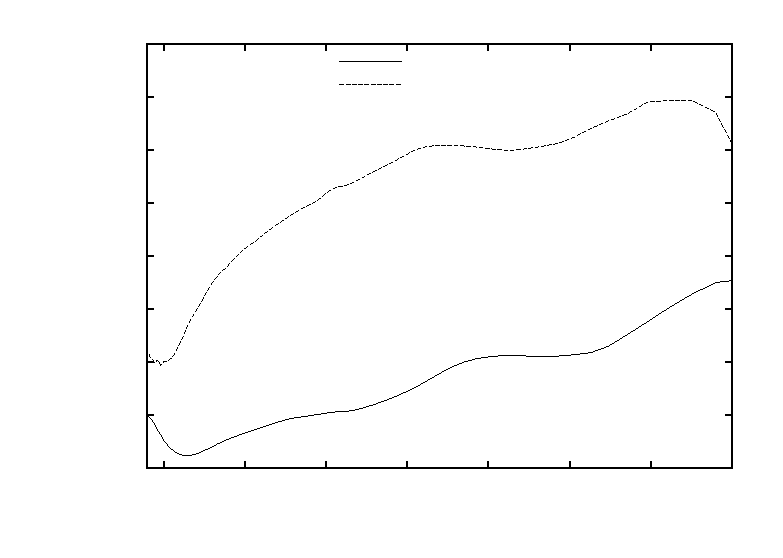
\includegraphics{CoFeSi1}}%
    \gplfronttext
  \end{picture}%
\endgroup

\caption{Spektrum vzorku CoFeSi1}
\label{sCoFeSi1}
\end{figure}

\begin{figure}
% GNUPLOT: LaTeX picture with Postscript
\begingroup
  \makeatletter
  \providecommand\color[2][]{%
    \GenericError{(gnuplot) \space\space\space\@spaces}{%
      Package color not loaded in conjunction with
      terminal option `colourtext'%
    }{See the gnuplot documentation for explanation.%
    }{Either use 'blacktext' in gnuplot or load the package
      color.sty in LaTeX.}%
    \renewcommand\color[2][]{}%
  }%
  \providecommand\includegraphics[2][]{%
    \GenericError{(gnuplot) \space\space\space\@spaces}{%
      Package graphicx or graphics not loaded%
    }{See the gnuplot documentation for explanation.%
    }{The gnuplot epslatex terminal needs graphicx.sty or graphics.sty.}%
    \renewcommand\includegraphics[2][]{}%
  }%
  \providecommand\rotatebox[2]{#2}%
  \@ifundefined{ifGPcolor}{%
    \newif\ifGPcolor
    \GPcolortrue
  }{}%
  \@ifundefined{ifGPblacktext}{%
    \newif\ifGPblacktext
    \GPblacktexttrue
  }{}%
  % define a \g@addto@macro without @ in the name:
  \let\gplgaddtomacro\g@addto@macro
  % define empty templates for all commands taking text:
  \gdef\gplbacktext{}%
  \gdef\gplfronttext{}%
  \makeatother
  \ifGPblacktext
    % no textcolor at all
    \def\colorrgb#1{}%
    \def\colorgray#1{}%
  \else
    % gray or color?
    \ifGPcolor
      \def\colorrgb#1{\color[rgb]{#1}}%
      \def\colorgray#1{\color[gray]{#1}}%
      \expandafter\def\csname LTw\endcsname{\color{white}}%
      \expandafter\def\csname LTb\endcsname{\color{black}}%
      \expandafter\def\csname LTa\endcsname{\color{black}}%
      \expandafter\def\csname LT0\endcsname{\color[rgb]{1,0,0}}%
      \expandafter\def\csname LT1\endcsname{\color[rgb]{0,1,0}}%
      \expandafter\def\csname LT2\endcsname{\color[rgb]{0,0,1}}%
      \expandafter\def\csname LT3\endcsname{\color[rgb]{1,0,1}}%
      \expandafter\def\csname LT4\endcsname{\color[rgb]{0,1,1}}%
      \expandafter\def\csname LT5\endcsname{\color[rgb]{1,1,0}}%
      \expandafter\def\csname LT6\endcsname{\color[rgb]{0,0,0}}%
      \expandafter\def\csname LT7\endcsname{\color[rgb]{1,0.3,0}}%
      \expandafter\def\csname LT8\endcsname{\color[rgb]{0.5,0.5,0.5}}%
    \else
      % gray
      \def\colorrgb#1{\color{black}}%
      \def\colorgray#1{\color[gray]{#1}}%
      \expandafter\def\csname LTw\endcsname{\color{white}}%
      \expandafter\def\csname LTb\endcsname{\color{black}}%
      \expandafter\def\csname LTa\endcsname{\color{black}}%
      \expandafter\def\csname LT0\endcsname{\color{black}}%
      \expandafter\def\csname LT1\endcsname{\color{black}}%
      \expandafter\def\csname LT2\endcsname{\color{black}}%
      \expandafter\def\csname LT3\endcsname{\color{black}}%
      \expandafter\def\csname LT4\endcsname{\color{black}}%
      \expandafter\def\csname LT5\endcsname{\color{black}}%
      \expandafter\def\csname LT6\endcsname{\color{black}}%
      \expandafter\def\csname LT7\endcsname{\color{black}}%
      \expandafter\def\csname LT8\endcsname{\color{black}}%
    \fi
  \fi
  \setlength{\unitlength}{0.0500bp}%
  \begin{picture}(7200.00,5040.00)%
    \gplgaddtomacro\gplbacktext{%
      \csname LTb\endcsname%
      \put(1078,704){\makebox(0,0)[r]{\strut{}-0.3}}%
      \put(1078,1156){\makebox(0,0)[r]{\strut{}-0.25}}%
      \put(1078,1609){\makebox(0,0)[r]{\strut{}-0.2}}%
      \put(1078,2061){\makebox(0,0)[r]{\strut{}-0.15}}%
      \put(1078,2513){\makebox(0,0)[r]{\strut{}-0.1}}%
      \put(1078,2966){\makebox(0,0)[r]{\strut{}-0.05}}%
      \put(1078,3418){\makebox(0,0)[r]{\strut{} 0}}%
      \put(1078,3870){\makebox(0,0)[r]{\strut{} 0.05}}%
      \put(1078,4323){\makebox(0,0)[r]{\strut{} 0.1}}%
      \put(1078,4775){\makebox(0,0)[r]{\strut{} 0.15}}%
      \put(1379,484){\makebox(0,0){\strut{} 1.5}}%
      \put(2227,484){\makebox(0,0){\strut{} 2}}%
      \put(3074,484){\makebox(0,0){\strut{} 2.5}}%
      \put(3922,484){\makebox(0,0){\strut{} 3}}%
      \put(4769,484){\makebox(0,0){\strut{} 3.5}}%
      \put(5617,484){\makebox(0,0){\strut{} 4}}%
      \put(6464,484){\makebox(0,0){\strut{} 4.5}}%
      \csname LTb\endcsname%
      \put(176,2739){\rotatebox{-270}{\makebox(0,0){\strut{}Polární Kerrův jev [deg.]}}}%
      \put(4006,154){\makebox(0,0){\strut{}$E$ [eV]}}%
    }%
    \gplgaddtomacro\gplfronttext{%
      \csname LTb\endcsname%
      \put(5816,1537){\makebox(0,0)[r]{\strut{}$\theta_K$}}%
      \csname LTb\endcsname%
      \put(5816,1317){\makebox(0,0)[r]{\strut{}$\epsilon_K$}}%
      \csname LTb\endcsname%
      \put(5816,1097){\makebox(0,0)[r]{\strut{}$\theta_K$}}%
      \csname LTb\endcsname%
      \put(5816,877){\makebox(0,0)[r]{\strut{}$\epsilon_K$}}%
    }%
    \gplbacktext
    \put(0,0){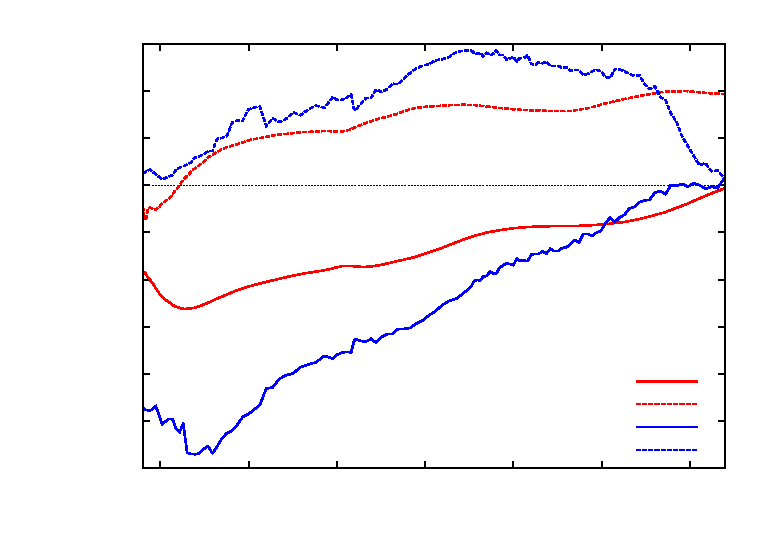
\includegraphics{CoFeSi2}}%
    \gplfronttext
  \end{picture}%
\endgroup

\caption{Spektrum vzorku CoFeSi2}
\label{sCoFeSi2}
\end{figure}
